\documentclass[a4paper,11pt,twoside]{article}
\usepackage[utf8]{inputenc}
\usepackage[german]{babel}
\usepackage{graphicx}
\usepackage{subcaption}
\usepackage{wrapfig}
\usepackage{hyperref}
\usepackage{float}
\usepackage{textcomp}
\usepackage[left=2.00cm, right=2.00cm, top=4.00cm, bottom=3.00cm]{geometry}
\usepackage{fancyhdr}
\renewcommand{\familydefault}{\sfdefault}
\pagestyle{fancy}
\fancyhf{}
\fancyhead[RE,RO]{\large Autor:Jinyao Zhu, Datum:28.01.2019}
\fancyhead[LE,LO]{\large Inbetriebnahmeanleitung - Tag my Plant}
\fancyfoot[RE,RO]{\thepage}

\renewcommand{\headrulewidth}{2pt}
\renewcommand{\footrulewidth}{1pt}

\usepackage{color}
\usepackage{listings}
\definecolor{maroon}{rgb}{0.5,0,0}
\definecolor{darkgreen}{rgb}{0,0.5,0}
\lstdefinelanguage{XML}
{
	basicstyle=\ttfamily,
	morestring=[s]{"}{"},
	morecomment=[s]{?}{?},
	morecomment=[s]{!--}{--},
	commentstyle=\color{darkgreen},
	moredelim=[s][\color{black}]{>}{<},
	moredelim=[s][\color{red}]{\ }{=},
	stringstyle=\color{blue},
	identifierstyle=\color{maroon}
}

\begin{document}

\begin{flushleft}
	
	\Large \textbf{Inbetriebnahmeanleitung}
\end{flushleft}

\section{ENTWICKLUNGSUMGEBUNG}
\subsection{Plattform}
\begin{itemize}
	\item Windows 10 Home 64 bit
\end{itemize}
\subsection{Verwendete Software}
\textbf{PC}:
\begin{itemize}
	\item Adobe PhoneGap Desktop 0.4.5 (BETA)
	\item Adobe PhoneGap Build (Cloud)
	\item VS Code (nicht erforderlich)
\end{itemize}
\textbf{Smartphone}:
\begin{itemize}
	\item Adobe PhoneGap f"ur Android (aus Google Play)
\end{itemize}

\section{STRUKTUR DER VERZEICHNISSE}
Alle Dateien bzw. Quellcode werden im Ordner \texttt{source/} gelegen.
\begin{itemize}
	\item \texttt{css/}: einige benutzerdefinierte Stylings f"ur der UI. 
	\item \texttt{html/}: beinhalte alle html Seite f"ur die Applikation.
	\item \texttt{img/}: Bilder f"ur die Applikation (nicht Datenbank relevant).
	\item \texttt{js/}: beinhalt app.js, JavaScript-Quellcode f"ur die Applikation Logik.
	\item \texttt{lib/}: verwendete Bibliotheken, Onsen-UI, jquery, Pdf.js. 
	\item \texttt{res/}: Icon f"ur die Applikation, z.B. App Icons, Splashs.
	\item \texttt{config.xml}: Konfiguration f"ur PhoneGap/PhoneGap Build, z.B. Plugins, Icons, Splashs und Erlaubnis zum Internet.
	\item \texttt{index.html}: Eingang f"ur PhoneGap / Startseite.
	\item \texttt{README.md}: Kurze Beschreibung und Anleitung.

\end{itemize}
\section{ERSTELLUNG DER PHONEGAP PROJEKT}
\subsection{Software Herunterladen}
PhoneGap Desktop f"ur Windows aus Internet herunterzuladen: \url{https://phonegap.com/products/}, und in Ihren Computer zu installieren.
\subsection{Neue PhoneGap Projekt erstellen}
\begin{itemize}
	\item Schritt 1: PhoneGap Desktop "offnen und Klicken Sie das ``\textbf{+}`` Zeichen (siehe Abbildung\ref{fig:preject1}).
\begin{figure}[h]
	\centering
	\minipage{0.35\textwidth}
	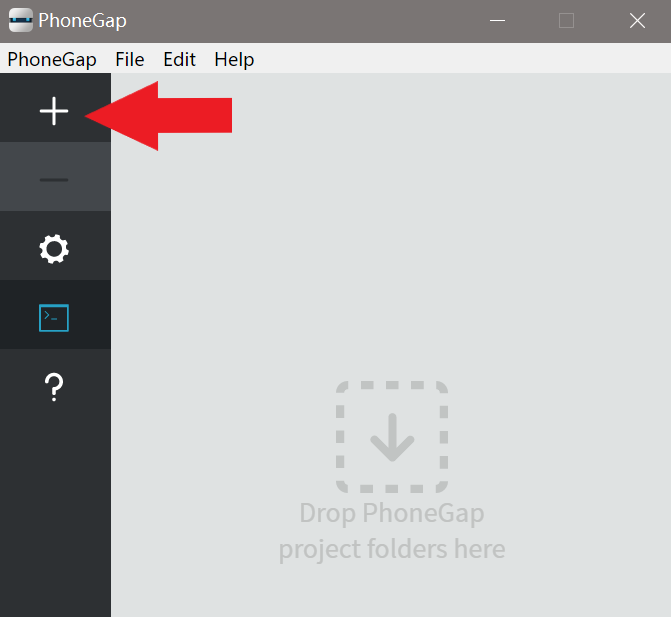
\includegraphics[width=\linewidth]{pic/project1}
	\caption{Schritt 1}\label{fig:preject1}
	\endminipage \hspace{2em}
	\minipage{0.405\textwidth}
	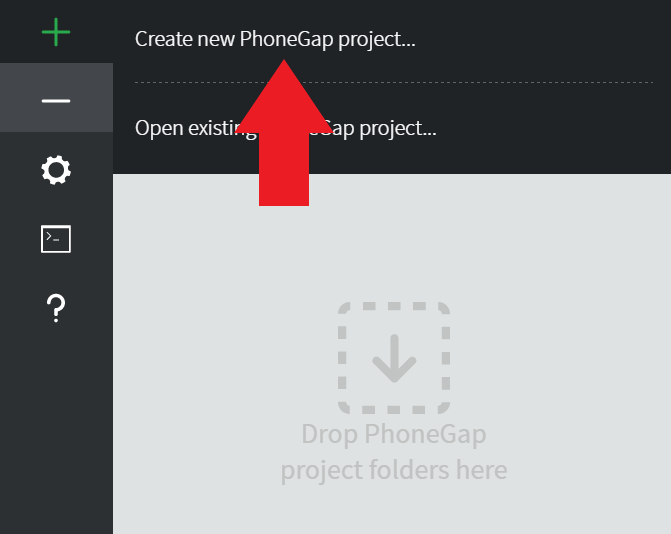
\includegraphics[width=\linewidth]{pic/project2}
	\caption{Schritt 2}\label{fig:preject2}
	\endminipage
\end{figure}
	\item Schritt 2: Klicken Sie ``\textbf{Create new PhoneGap project ...}`` (siehe Abbildung\ref{fig:preject2}).
	\item Schritt 3: W"ahlen Sie ``\textbf{Hello World}`` oder ``\textbf{Blank}``, dann Klicken "\textbf{Next}" (siehe Abbildung\ref{fig:preject3}).
	\item Schritt 4: W"ahlen Sie den ``\textbf{Local path}`` und geben Sie \textbf{Name} des Projektes (z.B. TagMyPlant), dann Klicken ``\textbf{Create project}`` (siehe Abbildung\ref{fig:preject4}).
	\begin{figure}[h]
		\centering
		\minipage{0.35\textwidth}
		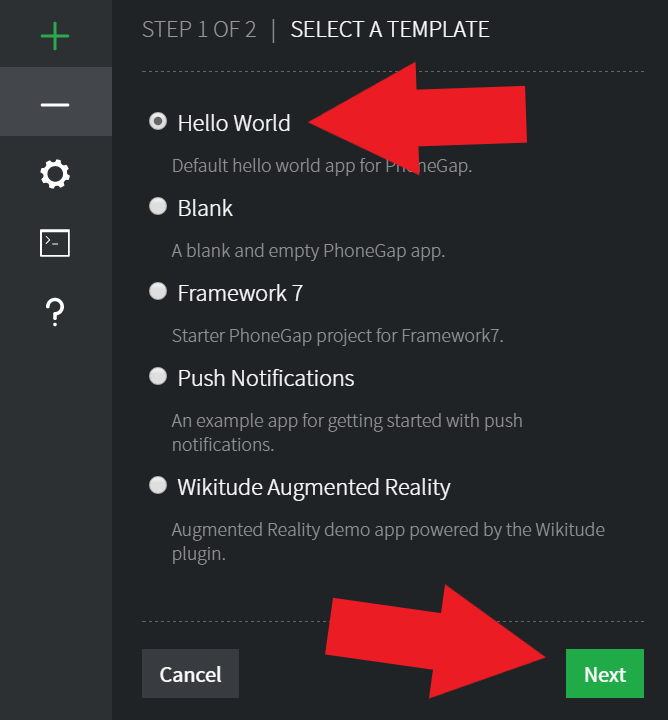
\includegraphics[width=\linewidth]{pic/project3}
		\caption{Schritt 3}\label{fig:preject3}
		\endminipage \hspace{2em}
		\minipage{0.358\textwidth}
		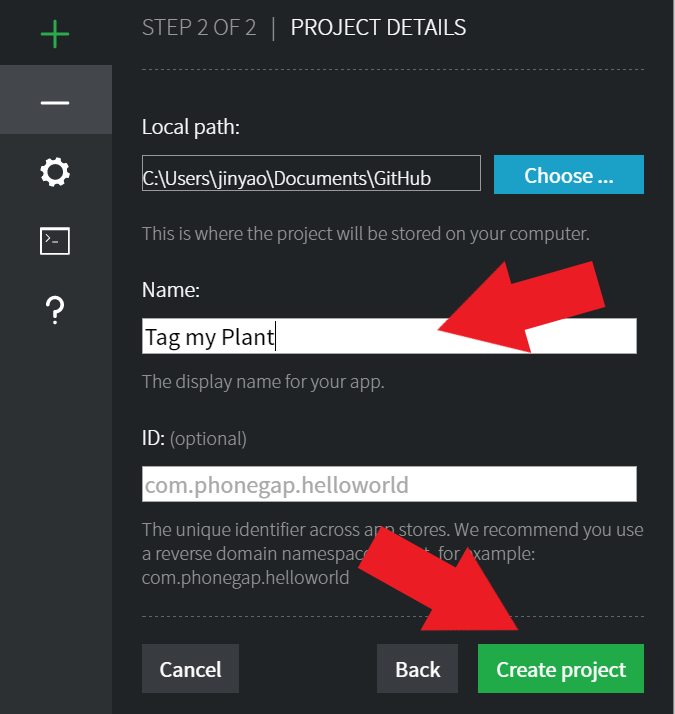
\includegraphics[width=\linewidth]{pic/project4}
		\caption{Schritt 4}\label{fig:preject4}
		\endminipage
	\end{figure}
	\item Schritt 5: "Offnen Sie den Ordner \texttt{www/} in root Ordner Ihres PhoneGap Projektes(z.B. \texttt{TagMyPlant/}), und entfernen Sie alle Dateien darin. Kopieren Sie alle Dateien von \texttt{source/}(aus Sektion 2), und sie in den \texttt{www/} Order des Projektes zu platzieren.
	\item Schritt 6: Kopieren Sie die \texttt{config.xml} in \texttt{www/}, und sie in root Ihres Projektes zu platzieren.
	\item Schritt 7: Starten Sie jetzt PhoneGap Desktop neu. Als erst Mal braucht das PhoneGap m"oglicherweise einige Minuten, um die Plugins zu laden. Wenn PhoneGap erfolgreich starten, werden die Adresse des Servers im unten gezeigt (siehe Abbildung \ref{fig:preject5}).
	\begin{figure}[h]
	\centering
	\minipage{0.35\textwidth}
	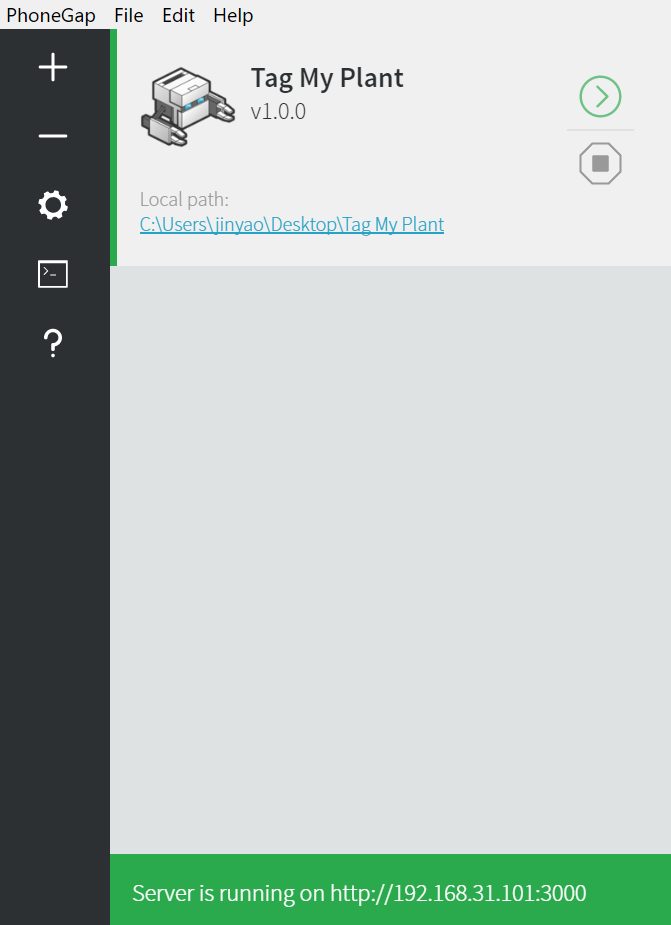
\includegraphics[width=\linewidth]{pic/project5}
	\caption{Schritt 7}\label{fig:preject5}
	\endminipage
	\end{figure}
	\item Schritt 8: "Offnen Sie jetzt PhoneGap in Ihrem Android Smartphone, geben Sie die Adresse ein. Beachten Sie, dass Ihrer Computer und Smartphone sich im dieselben lokalen Netzwerk befinden sollen. Wenn Sie mit dem Server erfolgreich verbunden haben, k"onnen Sie jetzt mit der Applikation spielen.
\end{itemize}

\section{ERSTELLUNG DER DATENBANK}
Die Datenbank besteht aus einem XML-Header und den Komponentendateien (siehe Abbildung \ref{fig:database1}). 
\begin{figure}[h]
	\centering
	\minipage{0.5\textwidth}
	
\includegraphics[width=\linewidth]{pic/database1}
	\caption{Dateien in der Datenbank}\label{fig:database1}
	\endminipage
\end{figure}

Der Ordner KVA-datasheet beinhaltet allen Dateien von den Komponenten, die von der Webseite des Institutes(\url{https://wiki.agtele.eats.et.tu-dresden.de/lib/exe/fetch.php?media=instructions:sample_plant:kva-datasheets.zip}) heruntergeladen werden kann. In \texttt{components.xml} werden Informationen von der Komponenten aufgezeichnet, z.B. Pfade zur Bilder, Pfade zum Datenblatt. Inhalt von components.xml sieht wie folgt aus:
\newpage
\lstset{language=XML}
\begin{lstlisting}
<?xml version="1.0" encoding="utf-8"?>
<CATALOG>
	<COMPONENT>
	  <NO>Y1</NO>
	  <NAME>2/2-way solenoid valve</NAME>
	  <PICTURE>KVA-datasheets/Y1/actuator_Y1_pic.PNG</PICTURE>
	  <DATASHEET>KVA-datasheets/Y1/170715_gb.pdf</DATASHEET>
	  <CODE>73871200</CODE>
	  <DESIGN>...</DESIGN>
	  <FUNCTION>...</FUNCTION>
	  <NOTE>...</NOTE>
	</COMPONENT>
	... <!-- andere Komponenten -->
</CATALOG>	
\end{lstlisting}

Die Inhalte von \texttt{<PICTURE>}, \texttt{<DATASHEET>}, \texttt{<CODE>} sind erforderlich, und muss mit der Tatsache entsprechen. Wenn Sie den \texttt{component.xml} ausgearbeitet haben, komprimieren Sie die Datenbank in eine ZIP-Datei, und laden Sie die ZIP-Datei auf Ihren Server hoch. Zum Testzweck  k"onnten Sie die Datenbank in Ihr Github-Konto hochladen. (Beachten: In diesem Fall m"ussen Sie nicht die Datenbank in ZIP-Datei komprimieren, und Sie sollen neue repository in Ihrem Github-Konto erstellen, dann die components.xml und die entsprechende Komponenten Datei hinzuzuf"ugen. Sie k"onnen die URL Ihre ZIP-Datei in Ihre Git repository bekommen,siehe Abbildung \ref{fig:database2}). Dabei \texttt{<CODE>} und \texttt{<NO>} zweier Komponenten m"ussen nicht identisch gesetzt werden.
\begin{figure}[h]
	\centering
	\minipage{0.7\textwidth}
	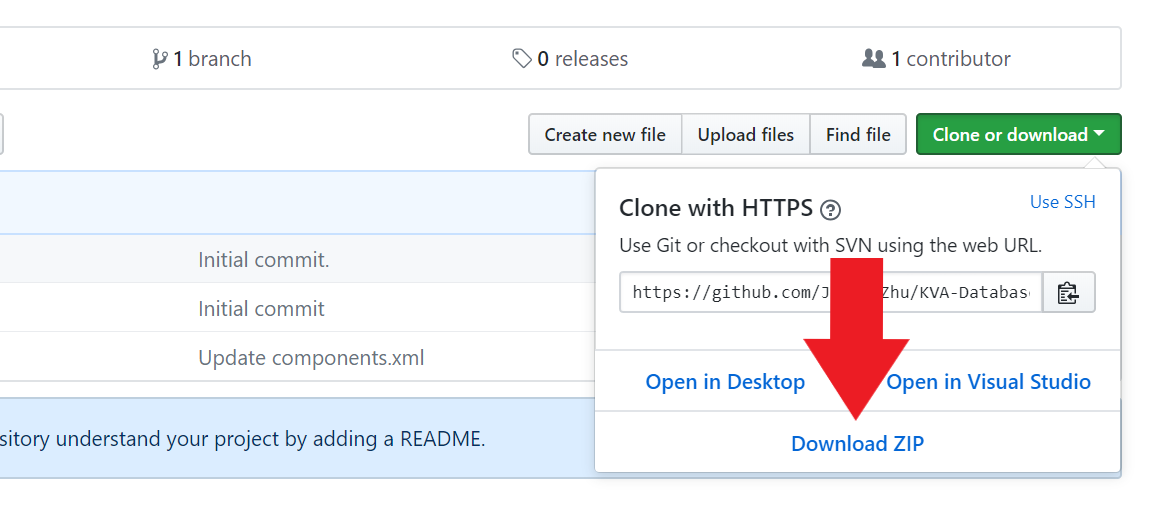
\includegraphics[width=\linewidth]{pic/database2}
	\caption{Dateien in der Datenbank}\label{fig:database2}
	\endminipage
\end{figure}

Jetzt k"onnen Sie die Adresse Ihrer ZIP-Datei in die Applikation(in der Einstellungsseite) eingeben. Beachten Sie auch, dass in der Applikation der relative Pfad zu root der Datenbank eingegeben werden muss. Dieser Pfad bezeichnet sich als der relative Pfad von der root Ihre ZIP-Datei zur root der Datenbank. Es gibt auch ausf"uhrliche Beispiel in der Hilfeseite der Applikation. 

Zur Testzweck k"onnen Sie diese Adresse benutzen: \url{https://github.com/JinyaoZhu/KVA-Database/archive/master.zip}, der relative Pfad ist: \texttt{KVA-Database-master/}. (Beachten:diese Adresse k"onnten in der Zukunft ung"ultig sein)

Es k"onnte sein, dass der Zugriff auf den Server eine Genehmigung erfordert. In diesem Fall k"onnen Sie in der Quellcode (die der Funktion \texttt{download()} in Zeile 584) die Genehmigungsinformation hinzuf"ugen.

\section{DIE QUELLCODE}
Die HTML-Dateien, die f"ur die Entwicklung relevant sind, sind in dem Ordner \texttt{html/} gelegt(au"serhalb der \texttt{index.html}). Und alle die Applikation relevante JavaScript-Funktionen sind in der \texttt{app.js} in \texttt{js/} definiert. F"ur weitere Entwicklungen k"onnen Sie \texttt{app.js} durchlesen.

\section{BUILD UND TESTEN}
\subsection{Build}
Zum Kompilieren der Quellcode zu einer APK-Datei k"onnen Sie PhoneGap Build nutzen. Er ist ein Online-Compiler, daher brauchen Sie eine Konto(kostenlos) von Adobe PhoneGap Build(\url{https://build.phonegap.com/}). Komprimieren Sie den Ordner \texttt{www/} in Ihrem PhoneGap Projekt in eine ZIP-Datei, dann die ZIP-Datei auf PhoneGap Build hochzuladen. Nach einigen zehn Sekunden wird ein APK-Paket generiert, laden Sie das herunter und installieren Sie das in Ihrem Smartphone. Nachdem Sie k"onnen die Applikation testen. Sie k"onnen auch das APK-Paket lokal generieren, zum Detail schauen Sie sich PhoneGap CLI an \url{http://docs.phonegap.com/references/phonegap-cli/}.
\subsection{Testen}
\subsubsection*{OPC XML-DA Server}
Wenn Sie mit dem OPC XML-DA Server verbinden m"ochten, stellen Sie einfach die Adresse in der Einstellungsseite ein.
\subsubsection*{Verbinden mit Barcode-Scanner(KDC300)}
Sie k"onnen die Benutzeranleitung f"ur KDC300 in dieser Webseite finden: \url{https://www.koamtac.com/wp-content/uploads/KDC.Reference.Manual.English.3.07.Rev0_.3.pdf}. Zur Kopplung "uber Bluetooth mit Ihrem Smartphone k"onnen Sie die ``Up-Button`` und ``Down-Button`` des Scanner gleichzeitig drucken, dann wird das Men"u von KDC300 gezeigt. In dem Men"u w"ahlen Sie \textbf{BT Service}\textbf{\textrightarrow}\textbf{Pairing}, dann ist der Scanner f"ur die Kopplung bereit. Scannen Sie mit Ihrem Smartphone den Scanner, dann ein Verbindung herzustellen.
\subsubsection*{Barcode/QR-Code}
Beim Benutzung des Scanners mit der Applikation brauchen Sie Barcodes/QR-Codes, die Ihre Datenbank entsprechend sind. Die Applikation ist nicht von dem Typ des Barcodes abh"angig, sobald der gescannte Code mit dem \texttt{<CODE>} in der Datenbank identisch ist. Es gibt viele Methode, Barcode/QR-Code zu erzeugen, Sie k"onnen Barcodes z.B. online generieren, bei dieser Webseite: \url{https://barcode.tec-it.com/de/}.

\end{document}
